\documentclass[12pt, a4paper, oneside]{ctexart}
\usepackage{amsmath,extarrows, amsthm, amssymb, bm, graphicx, hyperref, geometry, mathrsfs,color}

\title{\huge\textbf{集合与实数集}}
\author{luojunxun}
\date{\today}
\linespread{2}%行间距
\geometry{left=2cm,right=2cm,top=2cm,bottom=2cm}%设置页面
\CTEXsetup[format={\Large\bfseries}]{section}%section左对齐

%定义环境
\newenvironment{Def}[1][def-name]{\par\noindent{\textit{(#1):}\small}}{\\\par}
\newenvironment{theorem}[1][Theorem-name]{\par\noindent \textbf{Theorem #1:}\textit}{\\\par}
\newenvironment{corollary}[1][corollary-name]{\par\noindent \textbf{Corollary #1:}\textit}{\\\par\vspace*{15pt}}
\newenvironment{lemma}[1][lemma-name]{\par\noindent \textbf{Lemma #1:}\textbf}{\\\par}
\renewenvironment{proof}{\par\noindent{\textit{Proof:}\small}}{\\\par}
\newenvironment{example}[1][example-name]{\par{\textbf{Example:}}}{\\\par}
\newenvironment{say}{\center{\textit{summary:}}}{\\\par}
\newenvironment{note}[1][note-name]{\par\textit{#1:}}{\\\par}
\newcommand{\qie}{\quad\&\quad}


\begin{document}




















\begin{figure}[p]

    \centerline{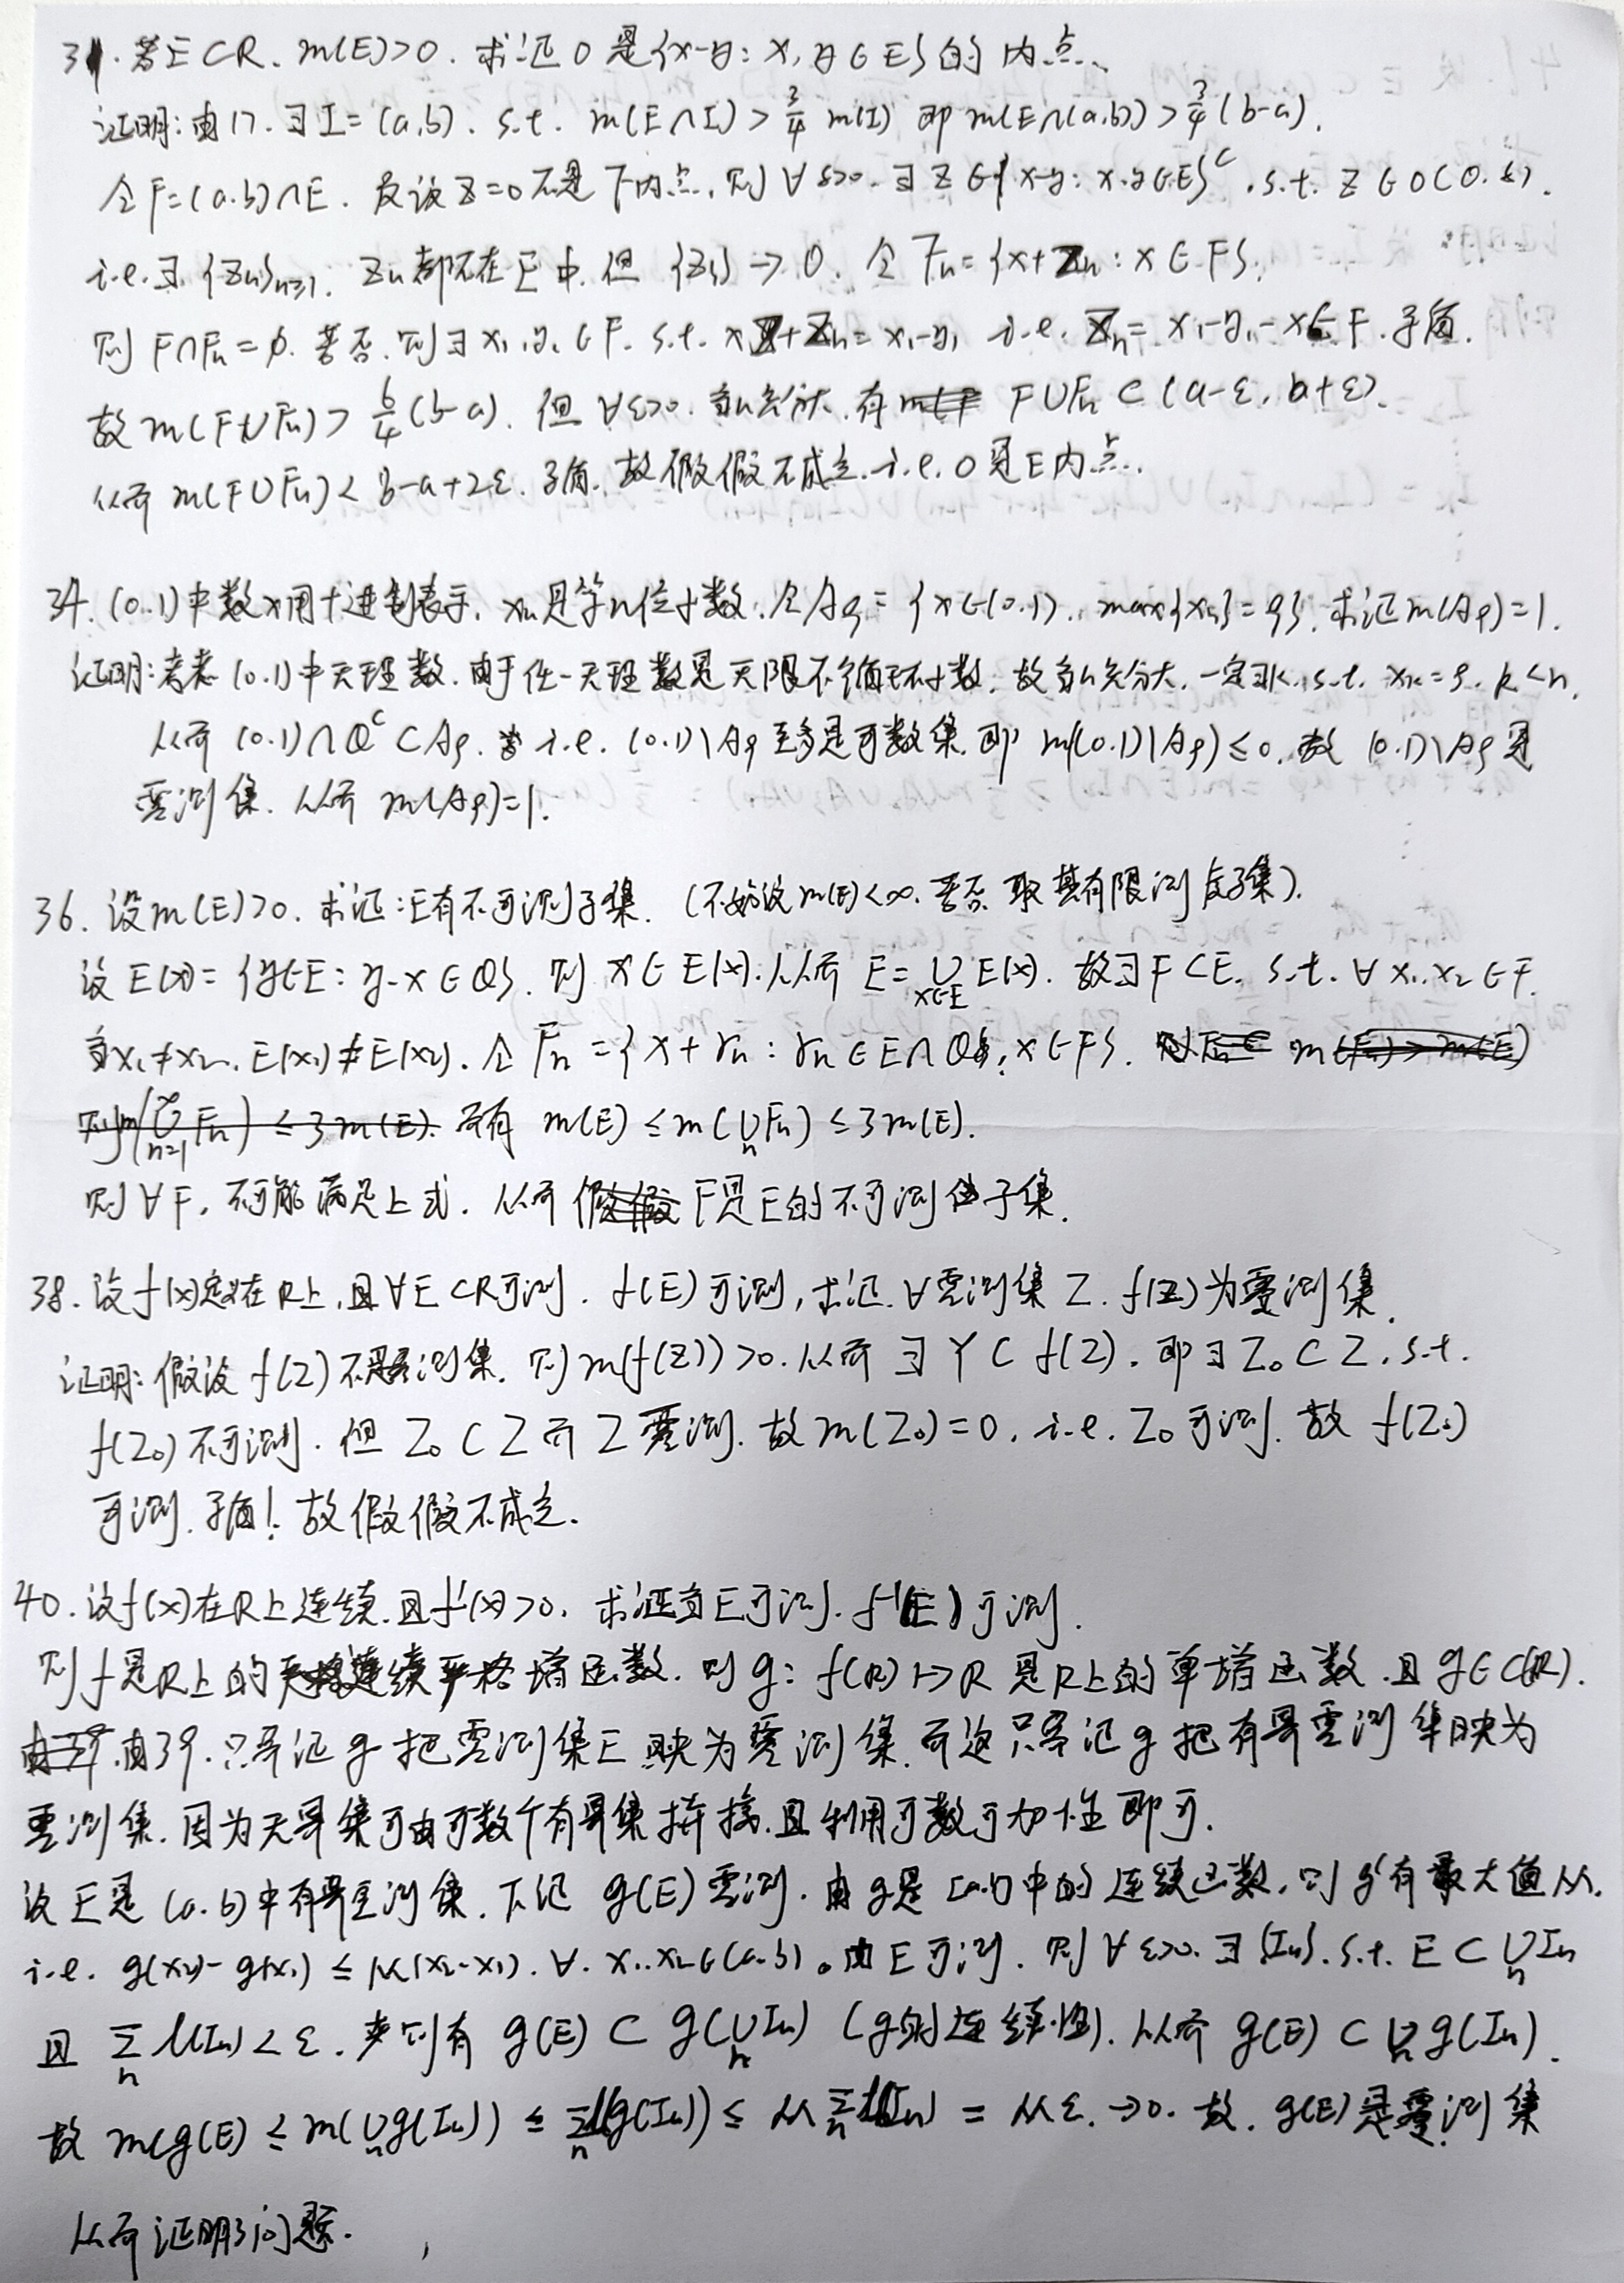
\includegraphics[width=1.2\linewidth,height=1.1\textheight]{RealFunction-7-1.jpg}}
\end{figure}

\begin{figure}[p]

    \centerline{\includegraphics[width=1.2\linewidth,height=1.1\textheight]{RealFunction-7-2.jpg}}
\end{figure}




% \bibliographystyle{IEEEtran}
% \bibliography{reference}



\end{document}